\documentclass[12pt,a4paper,english]{article}

\usepackage[left=2cm, top=3cm, text={17cm, 24cm}]{geometry} 
\usepackage[pdftex]{graphicx}
\usepackage{caption}
\usepackage{subfig}
\usepackage[utf8]{inputenc}
\usepackage{tabularx}
\usepackage[hyphens]{url}
\usepackage[unicode, colorlinks=true, hypertexnames=false, allcolors=blue]{hyperref}
\usepackage{xcolor}
\usepackage{times}
\usepackage{amsmath}
\usepackage{float}

\graphicspath{ {./images/} } 

\newcommand{\todo}[1]{\noindent\textcolor{red}{[[\textbf{TODO} \textbf{#1]]}}\\}
\newcommand{\phony}[1]{\textcolor{gray}{#1} \\}

\begin{document}
    \begin{titlepage}
        \begin{center}
            \vspace*{1cm}
        
            \begin{figure}[h!]
                
\includegraphics[scale=0.12]{VUT-FIT-logo-en.png}
            \end{figure}
            \vspace{1.5cm}

            \Large{\textbf{Epidemiological model on macro level}} \\
            \large{Modelling and Simulation}

            \vspace{0.5cm}
                
            \vspace{1.5cm}
            
            \textbf{Abramov Mikhail (xabram00)} \\
            \textbf{Pavel Yadlouski (xyadlo00)} 

            \vfill
                
            \vspace{0.8cm}
        
            Brno University of Technologies\\
            November, 2020
                
        \end{center}
    \end{titlepage}

    \tableofcontents
    \newpage

    \section{Introduction}
    The first aim of this project is to determine the possibilities for determining the value of the effectivity of various restrictive measures taken by the government of the Czech Republic for the period from September 1, 2020 till the last day of the project - December 5, 2020.

    The second aim is to create a predictive model for determining the number of persons who have illness in the same time, persons who have been ill or otherwise have immunity

    Used model contains different scenarios of quarantine precautions (using different types of lockdown).
    Based on simulations of this scenarios, influence of particular scenario is shown. 
    As an experiment, theoretical scenarios from the article and current lockdown type in Czech Republic are analyzed.

    \subsection{Contributors}    
    This project is solved by team of two students: Abramov Mikhail and Pavel 
    Yadlouski.
    
    \subsection{Model validation}
    Results of theoretical scenarios simulation are compared with reference results from the article. 
    The article by itself was subjected to critical analysis and minor formulas adjustments.
    Experiment with lockdown type in Czech Republic is compared with reality based on statistics values.
    
    \section{Topic analysis}

    As epidemic situation in the world become worth with time, there is need to take appropriate precautions based on mathematical models and simulation.
    Epidemiological model can be described as by stochastic as by deterministic model.
    Stochastic model can describe epidemics on micro level.
    For example on micro level time period between visitors came to the market is stochastic.
   
    But on macro level with large populations epidemics is described using deterministic model.
    In this model each individual of the population is assigned to different subgroup.
    And each subgroup represents a specific stage of the epidemic.
    The transition rates from one class to another are mathematically expressed as derivatives, this way model is defined by differential equations.
    In any time of the simulation following equation should valid:
    \begin{equation}
        \label{primary_question}
        P = \sum_{n = 1}^{n} S^t_n
      \end{equation}
    where $P$ is size of initial and $S^t_n$ is size of the subgroup $S_n$ in the time $t$. 

    One of the base mathematical model for simulation of expansion of the epidemic is SIR\footnote{\href{https://en.wikipedia.org/wiki/Compartmental\_models\_in\_epidemiology}{https://en.wikipedia.org/wiki/Compartmental\_models\_in\_epidemiology}} model. 
    SIR model is the simplest compartment methods that can be extended using different methodologies.
    This method compares three values:
    \begin{enumerate}
        \item \textbf{S} -- the number of \textbf{s}usceptible individuals
        \item \textbf{I} -- the number of \textbf{i}nfectious individuals.
        \item \textbf{R} -- the number of \textbf{r}emoved (and immune) or deceased individuals
    \end{enumerate} 

    \subsection{Sources}
    The necessary information to research this topic was found in scientific articles from IRCACS-International Research Center for Applied Complexity Sciences in  Colombia written by Danny Ibarra-Vega\cite{math_article}.

    \subsection{Approaches}
    For more complex view of system behavior, a mathematical model has been adopted with the Systems Dynamics(SD) methodology\footnote{\href{https://en.wikipedia.org/wiki/System\_dynamics}{https://en.wikipedia.org/wiki/System\_dynamics}}.
    The core of this methodology is that SD models solve the problem of simultaneity (mutual causation) by updating all variables in small time increments with positive and negative feedbacks and time delays structuring the interactions and control.
    
    Used SD model extends basic SIR model with separating the number of recovered and deceased individuals into two variables and addition of auxiliary and state variables that represent hospital capacity, contacts, contacts with infected. 
    As a result, there is a model of 4 stock variables and 4 corresponding differential equations (\ref{eq:quations}).

    \section{Concept model} \label{conc_model}
    In the model, we proceed from the assumption that immunity is stable and guarantees the absence of recurrent disease for the duration of research period. 
    
    \begin{center}
        \begin{figure}[ht!]
            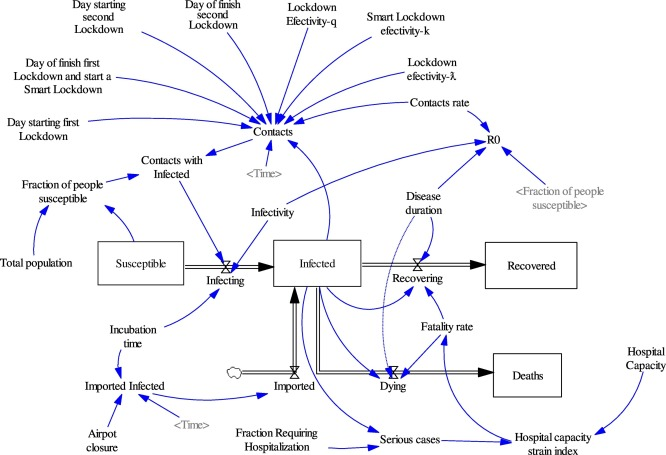
\includegraphics[scale=1]{1-s2.0-S0048969720324347-gr1.jpg}
            \caption{Stock and flows diagram}
            \label{fig:graph}
        \end{figure}
    \end{center}
    
    The diagram \ref{fig:graph}  from the reference article shows how each stock variable (susceptible, infectious, removed, deaths) is connected and influenced by other stock and auxiliary variable.
    Also 
    Auxiliary variables are constructed from bibliographic references or some estimated.
    
    \begin{table}[h!]
        \centering
        \begin{tabularx}{\textwidth}{|c|c|c|X|}
            \hline
            Name & Initial value & Units & Reference \\
            \hline
            Susceptible	                        & 100,000 &	People & Assumed\\
            Incubation time	                    & 5	 &  Days & Wu et al. (2020)\\
            Disease duration                    & 14	&  Days & Wu et al. (2020)\\
            Fraction requiring hospitalization	& 13  & \% & WHO report 73 (2020), Li et al. (2020) \\
            Infectivity	                        & 0.025 & Dimensionless & Estimated with RO \\
            Contacts rate	                    & 70   & Contacts/person & Assumed \\
            Hospital capacity	                & 1000 & Beds & Assumed \\
            Fatality rate	                    & 3	   & \% & WHO report 73 (2020), Wu et al. (2020) \\
            \hline
        \end{tabularx}
        \caption{Initial conditions \cite{math_article}}
        \label{tab:init_vars}
    \end{table}
    
    Meaning and notation of individual variable is explained in the table \ref{tab:not_var}

    \begin{table}[h!]
        \begin{center}
            \begin{tabular}{|c|c|c|}
                \hline
                Type of variable & Parameter & Notation \\
                \hline
                Auxiliary & Contacts rate                      & $\mu$  \\
                Auxiliary & Fatality rate                      & $Fr$ \\
                Auxiliary & Hospital capacity strain index     & $HiC$ \\
                Parameter & Incubation time                    & $it$ \\
                Parameter & Disease duration                   & $Dd$ \\
                Parameter & Fraction requiring hospitalization & $Fh$ \\
                Parameter & Infectivity                        & $\beta$ \\
                Parameter & Hospital capacity                  & $HC$ \\
                Parameter & Lockdown effectivity               & $\lambda$ \\
                Parameter & Smart lockdown effectivity         & $k$ \\
                Parameter & Post lockdown effectivity          & $q$ \\
                Parameter & Serious cases                      & $SC$  \\
                Parameter & Hospital capacity                  & $HC$ \\
                Stock     & Susceptible                        & $S$ \\
                Stock     & Infected                           & $I$ \\
                Stock     & Recovered                          & $R$ \\
                Stock     & Deaths                             & $D$ \\
                \hline
            \end{tabular}
        \end{center}
        \caption{Notation and variables \cite{math_article}}
        \label{tab:not_var}
    \end{table}

    Mathematical model of epidemic is
    \begin{subequations} \label{eq:quations}
        \begin{align*} 
            \frac{dS}{dt} &= - \frac{\beta Ci}{it}  \\ \\
            \frac{dI}{dt} &= \frac{\beta C}{it} - \frac{I}{Dd}\\ \\ % compaire with source question -> (1 - Fr) leads to poruseni of must have question 
            \frac{dR}{dt} &= \frac{I}{Dd} * (1 - Fr)\\ \\
            \frac{dD}{dt} &= \frac{I}{Dd} * (Fr)
        \end{align*}
    \end{subequations}

    During implementation of the model from the article, we found out that some variables in auxiliary equations are not defined in the article. 
    For example variable $F$ is not present in the article. 
    Using addition source article from Harvard University \cite{Harvard} we determined that variable $F$ is $Si$ divided on the total number of population $P$, otherwise we decided not to use additional variable for population and decided to use
    initial value of Susceptible as total population. 
    
    So, auxiliary equations that we used have following form
    \begin{subequations}
        \begin{align*} 
            Ci  &= C *F \\
            F   &= \frac{S}{S_{int}} \\ 
            HiC &= \frac{SC}{HC} \\
            SC  &= I * Fh \\
            Fr  &=    
            \begin{cases}
                3\% \; if \; HiC < 5 \\
                7\% \; if \; 5 < HiC < 30 \\
                10\% \; if \; HiC > 30
            \end{cases}
        \end{align*}
    \end{subequations}

    Influence of lockdown scenarios is described in the following way
    \begin{subequations}
        \begin{align*} 
            C  &=    
            \begin{cases}
                I * \mu \; if \; t \leq  t_1 \\
                I * \mu * \lambda \; if \; t_1 < t \leq t_2 \\
                I * \mu * k \; if \; t_2 < t \leq t_3 \\
                I * \mu * q \; if \; t_3 < t \leq t_4
            \end{cases}
        \end{align*}
    \end{subequations}

    There are 4 types of the lockdown:
    \begin{enumerate}
        \item without lockdown
        \item standard lockdown
        \item smart lockdown
    \end{enumerate}
    \noindent They are differ in effectivity of each one (parameters $\lambda$ and $k$ for standard and smart lockdown respectively). 
    In addition, there is parameter $q$ that shows post-lockdown effectivity.
    By effectivity we mean how much contact rate is reduced (in \%).

    \section{Experiment}
    At first, we conducted experiments from the source article.
    This experiments simulate different quarantine scenarios\footnote{In the source article there is diagram only for the first scenario (\ref{first_scen})}.

    \subsection{First scenario}
    \label{first_scen}
    In this scenario there is no lockdown at all.
    \begin{figure}[h!]
        \centering
        \subfloat[Result from the article]{
            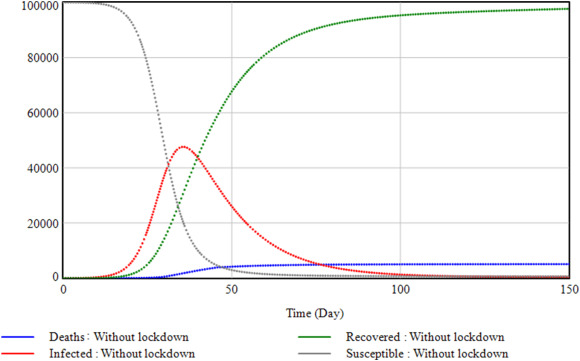
\includegraphics[width=0.45\textwidth]{without-lockdown.jpg}
        }
        \hfill
        \subfloat[Our result]{
            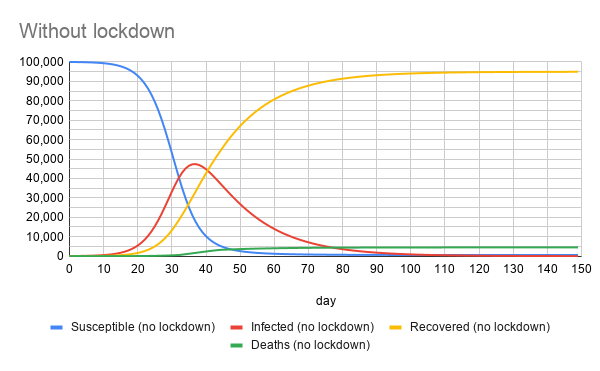
\includegraphics[width=0.45\textwidth]{without-lockdown-our.png}
        }
        \caption{Results of the first scenario}
    \end{figure}

    \subsection{Second scenario}
    \label{second_scenario}
    The second scenario includes one standard lockdown for 60 days from the 25th day after first beginning of the simulation till 85th day (long).
    \begin{itemize}
        \item 0 - 25 day -- no lockdown
        \item 26 - 85 day -- standard lockdown 
        \item 86 - 150 -- post-lockdown period
    \end{itemize}
    \begin{figure}[H]
        \centering
        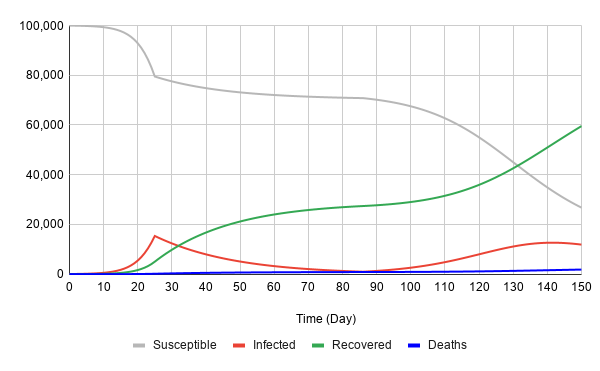
\includegraphics[scale=0.45]{1large.png}
        \caption{Results of the second scenario}
    \end{figure}

    \newpage
    \subsection{Third scenario}
    \label{third_scenario}
    In the third theoretical scenario there are two standard and one smart lockdown.
    Each lasts for 30 days (short).
    Smart lockdown acts between two standard lockdown.
    \begin{itemize}
        \item 0 - 25 day -- no lockdown
        \item 26 - 55 day -- standard lockdown 
        \item 56 - 85 day -- smart lockdown
        \item 86 - 115 -- standard lockdown
        \item 116 - 150 -- post-lockdown period
    \end{itemize}
    \begin{figure}[h!]
        \centering
        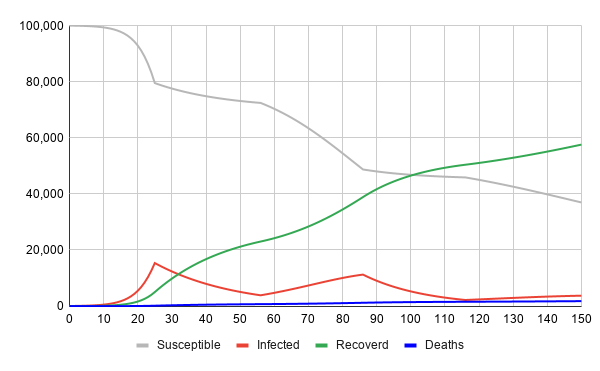
\includegraphics[scale=0.55]{2short+smart.png}
        \caption{Results of the third scenario}
    \end{figure}
    
    \subsection{Fourth scenario}
    \label{fourth_scenario}
    In the last theoretical scenario there is only two lockdown: one standard and one smart.
    Each lasts for 40 days (medium).
    \begin{itemize}
        \item 0 - 25 day -- no lockdown
        \item 26 - 65 day -- standard lockdown 
        \item 66 - 105 day -- smart lockdown
        \item 106 - 150 -- post-lockdown period
    \end{itemize}
    \begin{figure}[h!]
        \centering
        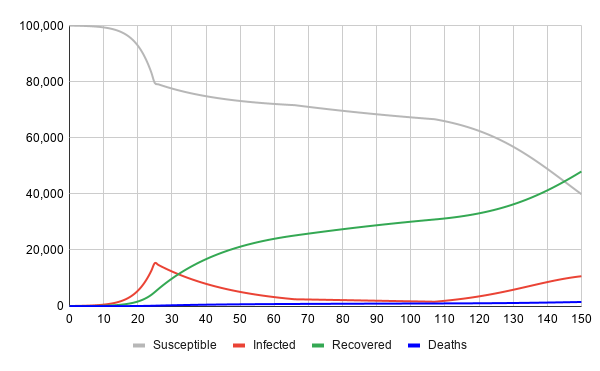
\includegraphics[scale=0.55]{med+smart.png}
        \caption{Results of the fourth scenario}
    \end{figure}
    
    \newpage
    \subsection{Our experiment}

    The purpose of our experiment was to determine the level of measures effectivity  taken by the government of the Czech Republic to counter covid19.
    
    Data provided by the information portal of the Ministry of Health (https://onemocneni-aktualne.mzcr.cz/covid-19) 
    were used as reference materials to compare model with real situation.
    
    \begin{table}[h!]
        \centering
        \begin{tabularx}{\textwidth}{|c|c|c|X|}
            \hline
            Name & Initial value & Units & Reference \\
            \hline
            Susceptible	                        & 10,680,000 &	People & Statistics \\
            Infected                            & 4,917 &	People & Statistics \\
            Recovered                           & 19,783 &	People & Statistics \\
            Deaths                              & 428 &	People & Statistics \\
            Incubation time	                    & 5	 &  Days & Wu et al. (2020)\\
            Disease duration                    & 14	&  Days & Wu et al. (2020)\\
            Fraction requiring hospitalization	& 13  & \% & WHO report 73 (2020), Li et al. (2020) \\
            Infectivity	                        & 0.025 & Dimensionless & Estimated with RO \\
            Contacts rate	                    & 29   & Contacts/person & Assumed \\
            Hospital capacity	                & 74760 & Beds & Statistics \\
            Fatality rate	                    & 1.7	   & \% & Assumed \\
            \hline
        \end{tabularx}
        \caption{Initial conditions}
        \label{tab:init_vars2}
    \end{table}
    
    The reasons for the change in the movement of the model are the measures introduced by the Government. In the model, we abstract
    from weather factors, because it is already obvious that in the warm summer time the virus slows down its spread.
    We also assume that every measure to reduce the spread of coronavirus cannot have negative effectivity. And also we abstract from the differences in social groups and population heterogeneity.
    
    \todo{Pasha poprav' ssylochki prosim suda}
    Investigated measures and model time intervals:
    \begin{itemize}
        \item 0 - 9   day -- no measures, setting the basic parameters of the model: Fatality rate, Contacts rate
        \item 10 - 20 day -- indoor mandatory  masks (https://www.mzcr.cz/tiskove-centrum-mz/od-ctvrtka-budou-povinne-rousky-ve-vnitrnich-prostorach-budov-v-cele-cr/)
        \item 21 - 33 day -- distance education in universities (First prague) (https://www.idnes.cz/zpravy/domaci/koronavirus-covid-19-aktualizace-semafor-praha-cesko.A200921_181218_domaci_lesa)
        \item 34 - 37 day -- distance education in all universities  (https://apps.odok.cz/djv-agenda?date=2020-09-30)
        \item 38 - 40 day -- sports and recreation facilities are closed. (https://www.lidovky.cz/domov/zive-vlada-projednala-nova-covidova-opatreni-kabinet-informuje-jake-restrikce-cekaji-cesko.A201008_110950_ln_domov_sei)
        \item 41 - 49 day -- distance education in schools (https://koronavirus.mzcr.cz/vlada-od-stredy-zprisni-preventivni-opatreni-posle-ochranne-pomucky-invalidnim-duchodcum)
        \item 50 - 56 day -- outdoor mandatory masks, shops and restaurants are closed (https://www.kurzy.cz/zpravy/562948-od-stredy-21-rijna-do-odvolani-rousky-vsude-v-kontaktu-s-dalsi-osobou-i-venku/ , https://prachaticky.denik.cz/zpravy_region/zavreni-obchodu-i-sluzeb-obchodnici-se-obavaji-financnich-problemu-20201021.html)
        \item 57 - 77 day -- imposed curfew (https://www.denik.cz/z_domova/cesko-narizeni-aktualne-omezeni-20201028.html)
        \item 78 - 92 day -- PES4 (https://onemocneni-aktualne.mzcr.cz/pes)
        \item 93 - XX day -- PES3 (https://www.vlada.cz/cz/media-centrum/aktualne/do-tretiho-stupne-pes-prejde-cesko-ve-ctvrtek--rozhodla-vlada-185260/)
    \end{itemize}
    
    \newpage
    \section{Conclusion} 
    \begin{figure}[H]
        \centering
        \subfloat[Result from the article]{
            \includegraphics[width=0.45\textwidth]{deaths.jpg}
        }
        \hfill
        \subfloat[Our result]{
            \includegraphics[width=0.45\textwidth]{deaths-our.png}
        }
        \caption{Deaths}
    \end{figure}

    \begin{figure}[H]
        \centering
        \subfloat[Result from the article]{
            \includegraphics[width=0.45\textwidth]{infected.png}
        }
        \hfill
        \subfloat[Our result]{
            \includegraphics[width=0.45\textwidth]{infected-our.png}
        }
        \caption{Infected}
    \end{figure}

    During implementation we met with serious inaccuracies that led to a difference in graphics
    \begin{itemize}
        \item \textbf{No initial values}\\ In the source article there is no initial value of Infected variable
        \item \textbf{Logical mistake in question}\\
        The model assumes that recovered person can't be infected again.
        In source model question for Infected variable has following form:
        $$\frac{dI}{dt} = \frac{\beta C}{it} - \frac{I}{Dd} * (1 - Fr)$$
        \noindent The problem is that factor $(1 - Fr)$ includes only recovered people, but not dead people. Logically dead person can't be infected again too :)
        This mistake leads to violation of primary question \eqref{primary_question}
    \end{itemize}

    After all the experiments, we came to the conclusion that the most effective  scenario is the fourth \eqref{fourth_scenario} based on count of deaths.

    \subsection{Conclusion of our experiment}

    According to the results obtained, the measures received the following percentage of effectivity (percentage decrease in the number of social contacts):
    \begin{itemize}
        \item 0 - 9   day -- no measures -- 0\% -- Total: 0\% 
        \item 10 - 20 day -- indoor mandatory  masks -- 5\% -- Total: 5\% 
        \item 21 - 33 day -- distance education in universities (first Prague) -- 1\% -- Total: 6\%
        \item 34 - 37 day -- distance education in all universities -- 1\% -- Total: 7\%
        \item 38 - 40 day -- sports and recreation facilities are closed -- 1\% -- Total: 8\%
        \item 41 - 49 day -- distance education in schools -- 3\% -- Total: 11\%
        \item 50 - 56 day -- outdoor mandatory masks, shops and restaurants are closed -- 15\% -- Total: 26\%
        \item 57 - 77 day -- imposed curfew -- 20\% -- Total: 46\%
        \item 78 - 92 day -- PES4 -- 25\% -- Total: 71\%
        \item 93 - XX day -- PES3 -- -35\% -- Total: 36\%
    \end{itemize}
    

    Next, we will consider two scenarios with a third and fourth level PES.
    
    We based our analysis on death and recovered values as on more statistically accurate.

    \todo{Pasha jobni kartinki prosim suda}
    
    Thus, we can say that measures by themselves cannot be effective. Measures can only be effective in combination. It is not enough to close universities and leave restaurants and bars open. The opposite is not enough too, when leaving schools and universities open.
    
     \todo{Pasha i ssylochku tut}
     
    Despite the fact that we did not have enough time to assess the decrease in the level of the PES system, we tried to predict two scenarios, from which it follows that it is necessary to maintain the fourth level of danger, which has been shown by the system itself (https: //www.novinky. cz / koronavirus / clanek / on-line-index-rizika-stoupl-zpet-do-ctvrteho-stupne-zbyva-jediny-bod-40344376).
    
    We also came to the conclusion that the actual mortality differs from the expected one and is 1.7% instead of 3%,
    which may be due to the increase in testing coverage and the emergence of treatment methods.

    We recommend a more systematic approach when introducing restrictive measures, 
    because it is often not so easy to determine which measure really influenced the improvement of the situation,
    at the moment the PES system can solve this problem, since it consolidates a number of measures at each level within itself and their application becomes systemic.
    \todo{Co se naucili}
    \todo{Doporuceni}    

    \clearpage
    \nocite{*}
	\bibliographystyle{abbrv}
	\bibliography{citation}
\end{document}